\section{Introduction}
\label{sec:introduction}

Give each unoriented nearest-neighbor edge $e$ of $\Z^2$ an independent
positive weight $\tau_e$. The cost $\tau(P)$ of a finite path is the sum
of its edge weights, counted with traversal multiplicity. Write
$\Delta P$ for its terminal vertex minus its initial vertex. Then
\[
 T(x,y)=\inf_{P:x\to y}\tau(P)
\]
is its passage time. All lattice paths in this definition are undirected.
For the laws considered here, the shape theorem gives a deterministic
norm $\mu$ on $\R^2$, characterized by
\[
 \frac{T(0,\lfloor tv\rfloor)}t\longrightarrow\mu(v)
 \quad\text{almost surely for each fixed }v\in\R^2.
\]
Its unit ball $\Bcal=\{v:\mu(v)\le1\}$ is the limit shape.
We write $|\cdot|$ for the Euclidean norm unless another norm is specified.

\begin{theorem}[The exponential limit shape]
\label{thm:exponential-shape}
For independent exponential edge weights of any rate $\lambda>0$,
the norm $\mu$ is Fr\'echet differentiable on $\R^2\setminus\{0\}$,
and its unit ball is strictly convex. In particular,
\[
 \mu((1-t)x+ty)<1
 \quad\text{if }x,y\in\partial\Bcal,\ x\ne y,\ 0<t<1,
\]
and $\partial\Bcal$ is a $C^1$ curve with a unique supporting line
at every point.
\end{theorem}

The differentiability argument applies to a larger family. For
$\kappa,\lambda>0$, the Gamma law of shape $\kappa$ and rate $\lambda$
has density
\[
 p_{\kappa,\lambda}(t)
 =\frac{\lambda^\kappa}{\Gamma(\kappa)}
   t^{\kappa-1}e^{-\lambda t},\qquad t>0.
\]
The exponential law is the case $\kappa=1$.

\begin{theorem}[Differentiability for Gamma weights]
\label{thm:gamma-differentiability}
For independent Gamma edge weights with any fixed shape $\kappa>0$
and rate $\lambda>0$, the norm $\mu$ is Fr\'echet differentiable at
every nonzero vector, and $\partial\Bcal$ is a $C^1$ curve.
\end{theorem}

Strict convexity and differentiability exclude different features of a
convex boundary: a flat face has more than one point on a supporting
line, whereas a corner has more than one supporting line at a point
(Figure~\ref{fig:geometry}). Theorem~\ref{thm:gamma-differentiability}
does not assume strict convexity. The proof of strict convexity in
Part~\ref{part:strict} uses the exponential law and is independent of
the differentiability proof.

\begin{figure}[ht]
\centering
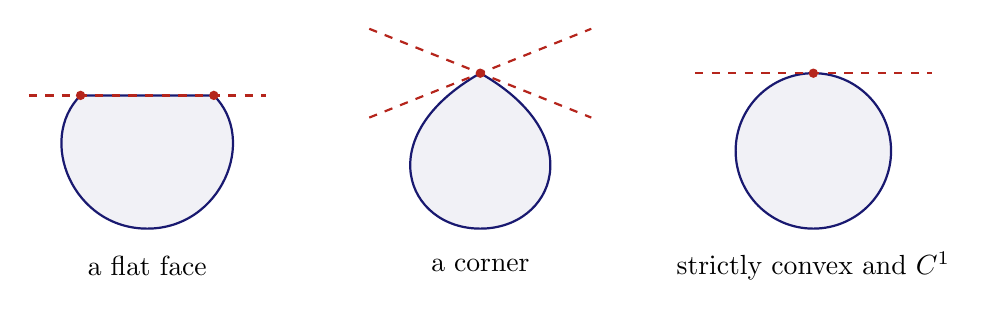
\begin{tikzpicture}[scale=0.94,line width=0.8pt,
  body/.style={draw=MidnightBlue,fill=MidnightBlue!6},
  support/.style={draw=BrickRed,dashed}]
 \begin{scope}[xshift=-4.5cm]
  \path[body] (-0.9,0.7)--(0.9,0.7)
   .. controls (1.5,0.1) and (1,-1.1) .. (0,-1.1)
   .. controls (-1,-1.1) and (-1.5,0.1) .. (-0.9,0.7);
  \draw[support] (-1.6,0.7)--(1.6,0.7);
  \fill[BrickRed] (-0.9,0.7) circle (1.8pt) (0.9,0.7) circle (1.8pt);
  \node at (0,-1.6) {a flat face};
 \end{scope}
 \begin{scope}
  \path[body] (0,1) .. controls (1.5,0.15) and (1,-1.1) .. (0,-1.1)
   .. controls (-1,-1.1) and (-1.5,0.15) .. (0,1);
  \draw[support] (-1.5,1.6)--(1.5,0.4);
  \draw[support] (-1.5,0.4)--(1.5,1.6);
  \fill[BrickRed] (0,1) circle (1.8pt);
  \node at (0,-1.6) {a corner};
 \end{scope}
 \begin{scope}[xshift=4.5cm]
  \path[body] (0,-0.05) circle (1.05);
  \draw[support] (-1.6,1)--(1.6,1);
  \fill[BrickRed] (0,1) circle (1.8pt);
  \node at (0,-1.6) {strictly convex and $C^1$};
 \end{scope}
\end{tikzpicture}
\caption{The two obstructions to regularity. These are schematic convex
bodies; the circle is not a proposed formula for the limit shape.}
\label{fig:geometry}
\end{figure}

\subsection{History and significance}

First-passage percolation was introduced by Hammersley and Welsh
\cite{HW1965}. The asymptotic-shape theory developed through the work of
Richardson \cite{Richardson1973} and Cox and Durrett \cite{CD1981},
alongside Kingman's ergodic theory of subadditive processes
\cite{Kingman1968}.
Although the shape theorem gives a convex deterministic body, its fine
geometry is much harder to determine; see the survey of Auffinger,
Damron, and Hanson \cite{ADH2017}. Theorem~\ref{thm:exponential-shape}
resolves positively the strict-convexity and differentiability
conjectures for the planar exponential model.

There are important partial results for both questions. Lalley
\cite{Lalley2003} gave sufficient conditions for strict convexity in
the standard lattice model, involving asymptotic straightness and
mean-zero scaling limits. In Richardson's site growth model, Durrett
and Liggett \cite{DurrettLiggett1981} established a flat edge for
parameters sufficiently close to one and identified its onset with the
threshold of a related contact process. For planar edge first-passage
percolation with support minimum normalized to one and an atom of mass $p$
there, Marchand \cite[Theorem~1.3]{Marchand2002} determined the exact
flat segment on the first-quadrant unit $\ell^1$ boundary when
$p>\vec p_c$, where $\vec p_c$ is the oriented-percolation threshold,
and a single diagonal contact point when $p=\vec p_c$. For finite-mean
laws in this class with $\vec p_c\le p<1$, Auffinger and Damron
\cite[Theorem~2.1]{AD13} proved differentiability at the endpoints,
including the critical contact point. These last two results concern
an atom at a positive minimum; exponential edge weights are nonatomic
and have essential infimum zero.

The connection between shape geometry and geodesics was developed by
Newman and Licea--Newman \cite{Newman1995,LiceaNewman1996}. Curvature
hypotheses and fixed-direction uniqueness play distinct roles in those
results. Damron and Hanson \cite{DH2017}
proved convergence and coalescence toward a specified supporting sector
under differentiability assumptions. Our two regularity conclusions
make that sector a single direction. Section~\ref{sec:consequences}
states the resulting geodesic and Busemann conclusions with the
direction fixed before the probability-one event is chosen. The
midpoint question of Benjamini, Kalai, and Schramm \cite{BKS2003}
is already answered qualitatively without shape regularity by Ahlberg
and Hoffman \cite{AH2019}. We explain its relation to the directional
results. For all Gamma laws, differentiability supplies infinitely
many extreme points, making the quantitative midpoint estimate of
Dembin, Elboim, and Peled \cite{DEP2024} applicable as well.

\subsection{Proof strategy}

\paragraph{Excluding a corner.}
Suppose two distinct extreme supporting functionals $f_-,f_+$ touch
the norm in a direction $u$, and let $f=(f_-+f_+)/2$. Their gap gives
a linear penalty for transverse motion. Part~\ref{part:differentiability}
turns this penalty into a positive excess over $f$ for every sufficiently
long simple path, contradicting the shape theorem along $u$.

First, a crossing confined to a long narrow strip is unlikely to save
a fixed multiple of the strip width over either extreme support.
Otherwise independent parallel trials, connected using one-sided
first-order contact with the norm, would yield macroscopic travel
below that support. Second, a finite-region change of measure produces
characteristic lengths $L$ for widths $s$, with $L/s\to\infty$ and
$L\le s^3$. Nested grids then extend the crossing estimate to arbitrary
endpoints, with a summable cost. Third, every cheap path chunk contains
a witness for a rare decreasing event. The van den Berg--Kesten
inequality \cite{BK85}, applied to disjoint edge witnesses, handles
repeated visits to the same coarse box and yields a bound for all
long simple paths at once. The counting builds on Kesten's rectangle
itineraries and crossing-multiplicity estimates
\cite[Section~3]{Kesten1980}; here the local witnesses certify negative
excess relative to a supporting functional.

The Gamma extension is built into this proof. Its distributional inputs
are exponential tails for short coordinate paths, a continuous quantile
representation for the witness inequality, and an exact likelihood
calculation: scaling one Gamma weight by $1-\delta$ gives likelihood
second moment $(1-\delta^2)^{-\kappa}$. Scaling $O(ns)$ weights with
$\delta$ of order $s/n$ has bounded second moment when $n=s^3$.
No differentiability or curvature estimate for $\mu$ enters these inputs.

\paragraph{Excluding a flat face.}
Under a hypothetical flat face, the stationary cocycle construction of
Damron and Hanson \cite{DH2014} supplies an additive random function
$B(x,y)$, with mean the supporting functional and with
$|B(x,y)|\le T(x,y)$. Thus a path from $x$ to $y$ has nonnegative
defect $\tau(P)-B(x,y)$. Part~\ref{part:strict} considers local random
paths, called roads, tracking two directions near the ends of the face.
At lattice scale $n$, let $b(n)$ be the infimum of a common upper bound
for their mean defect per period. A local perturbation gives
$b(n)\ge c_0>0$. The main construction gives a fixed integer $D$ and
$\rho<1$ such that
\[
 b(Dn)\le\rho b(n).
\]
Iteration contradicts the positive lower bound.

A finite-cell projection constructs local endpoint potentials
approximating increments of the generally nonlocal cocycle; interpolation
controls every possible attachment in a bounded road interval
(Section~\ref{found:sec-gauges}). A physical routing argument bounds the
savings obtainable from a selected collection of local shortcuts
(Proposition~\ref{access:collection}). An area-preserving deformation
then controls those savings along paths concentrated near an extreme
direction (Lemma~\ref{probability:thin-tails}). Passage-time concentration
and mean approximation estimates of Damron--Hanson--Sosoe \cite{DHS2014}
and Damron--Kubota \cite{DK2016} supply the quantitative metric input.

These estimates let a long geodesic toward an extreme endpoint supply
many crossings between neighboring walls while controlling the discarded
pieces. The extraction gives a small upper bound for the mean clipped
cost of a local crossing. Comparing this crossing with the current road, including the
short wall connections, transfers the clipped bound to a primary
candidate. To control the remaining large positive costs, a local rule
groups their flags into short clusters and traverses an independently
built spare road across each accepted cluster, with forward connections
at both ends (Lemma~\ref{improvement:replacement}). A matched cap controls
the frequency of flags, while separation and first-moment estimates
control the added cost. This reduces the full expected excess per road
period. A fixed rescaling restores the required tracking and locality,
so the improved paths belong to the class defining $b(n)$.

The two arguments use different endpoint corrections. In
Part~\ref{part:differentiability}, the deterministic defect
$\tau(P)-f(\Delta P)$ can be negative. In Part~\ref{part:strict}, the
cocycle defect is nonnegative on every forward subpath. Each part
introduces its own local coordinates and parameters.
